\begin{figure}[h]
	\centering
	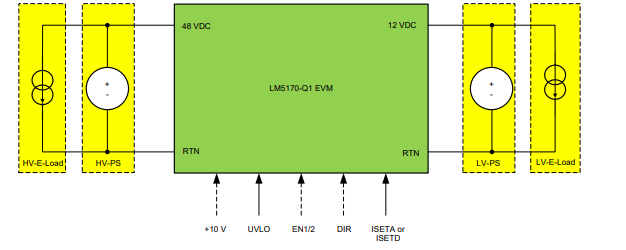
\includegraphics[width=1\textwidth]{Chap04/Figures/DC_DC_Converter_bench_setup.PNG}
	\caption{LM5170 DC/DC Converter Operation Setup \cite{TI_LM5170_BatteryTesting_Solution},\cite{TI_LM5170_EVM_User_Guide} }
	\label{fig:LM5170_DC_DC_Converter_Operation_Setup}
\end{figure}

\begin{equation}\label{eq:LTC_Pdissp_average}
    P_{DISS} = V_{IN} \times I_{LIMIT(MAX)}  = \left(24V \times 0.5A\right) = \left(6W\right)
\end{equation}

\begin{figure}[h]
	\centering
	\subfigure[MIFA antenna Gain Radiation pattern $@ \phi =90\deg$]{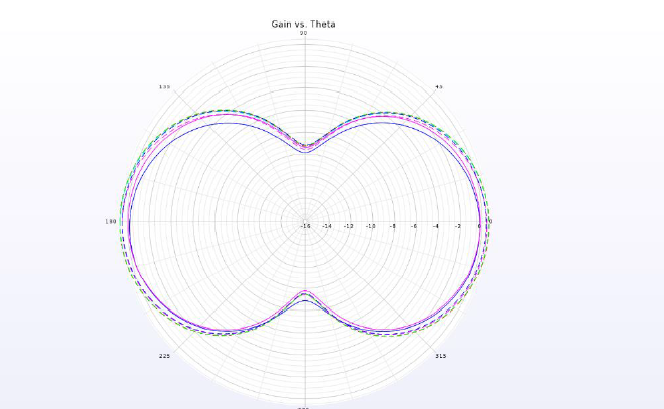
\includegraphics[scale=.5]{Chap03/Figures/mifa_Antenna_gain_pattern_phi_90.PNG}}
	\qquad
	\subfigure[MIFA antenna Gain Radiation pattern $@ \phi =0\deg$]{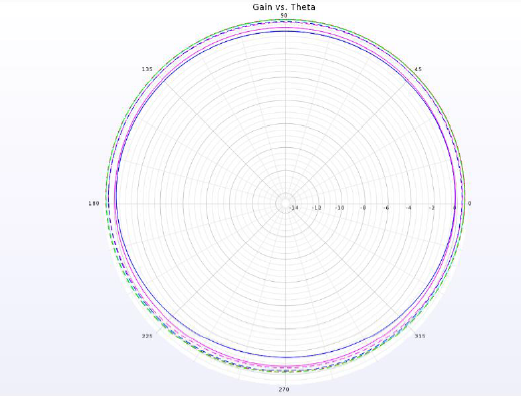
\includegraphics[scale=.5]{Chap03/Figures/mifa_Antenna_gain_pattern_phi_0.PNG}}
	\caption{MIFA Antenna Gain Radiation Pattren}
	\label{fig:MIFA_Antenna_Gain_Radiation_Pattren}
\end{figure}

\begin{enumerate}[(a)] % (a), (b), (c), ...
	\item
	\end{enumerate}
	.
	.
	.
	\begin{enumerate}[a)] % a), b), c), ...
	\item
\end{enumerate}



%%%%%%%%%%%%%% Cased Equation 

\begin{equation}
	f(x)=\begin{cases}
	  1, & \text{if $x<0$}.\\
	  0, & \text{otherwise}.
	\end{cases}
  \end{equation}


  \begin{table}[ht]
	\caption{Multi-column and multi-row table}
	\begin{center}
	\begin{tabular}{ccc}
		\hline
		\multicolumn{2}{c}{\multirow{2}{*}{Multi-col-row}}&X\\
		\multicolumn{2}{c}{}&X\\
		\hline
		X&X&X\\
		\hline
	\end{tabular}
	\end{center}
	\label{tab:multicol}
	\end{table}

	\begin{figure}
		\begin{subfigure}{.5\textwidth}
		  \centering
		  % include first image
		  \includegraphics[width=.8\linewidth]{log_demo1.png}  
		  \caption{Put your sub-caption here}
		  \label{fig:sub-first}
		\end{subfigure}
		\begin{subfigure}{.5\textwidth}
		  \centering
		  % include second image
		  \includegraphics[width=.8\linewidth]{log_demo2.png}  
		  \caption{Put your sub-caption here}
		  \label{fig:sub-second}
		\end{subfigure}
		
		\newline
		
		\begin{subfigure}{.5\textwidth}
		  \centering
		  % include third image
		  \includegraphics[width=.8\linewidth]{log_demo1.png}  
		  \caption{Put your sub-caption here}
		  \label{fig:sub-third}
		\end{subfigure}
		\begin{subfigure}{.5\textwidth}
		  \centering
		  % include fourth image
		  \includegraphics[width=.8\linewidth]{log_demo2.png}  
		  \caption{Put your sub-caption here}
		  \label{fig:sub-fourth}
		\end{subfigure}
		\caption{Put your caption here}
		\label{fig:fig}
		\end{figure}